% 杨氏双缝干涉实验

\pentry{双缝干涉中一个重要极限\upref{SltLim}}

用两个点波源作光的干涉实验的典型代表, 是杨氏实验.
\subsection{实验装置}
杨氏实验的装置如下图所示,
\begin{figure}[ht]
\centering
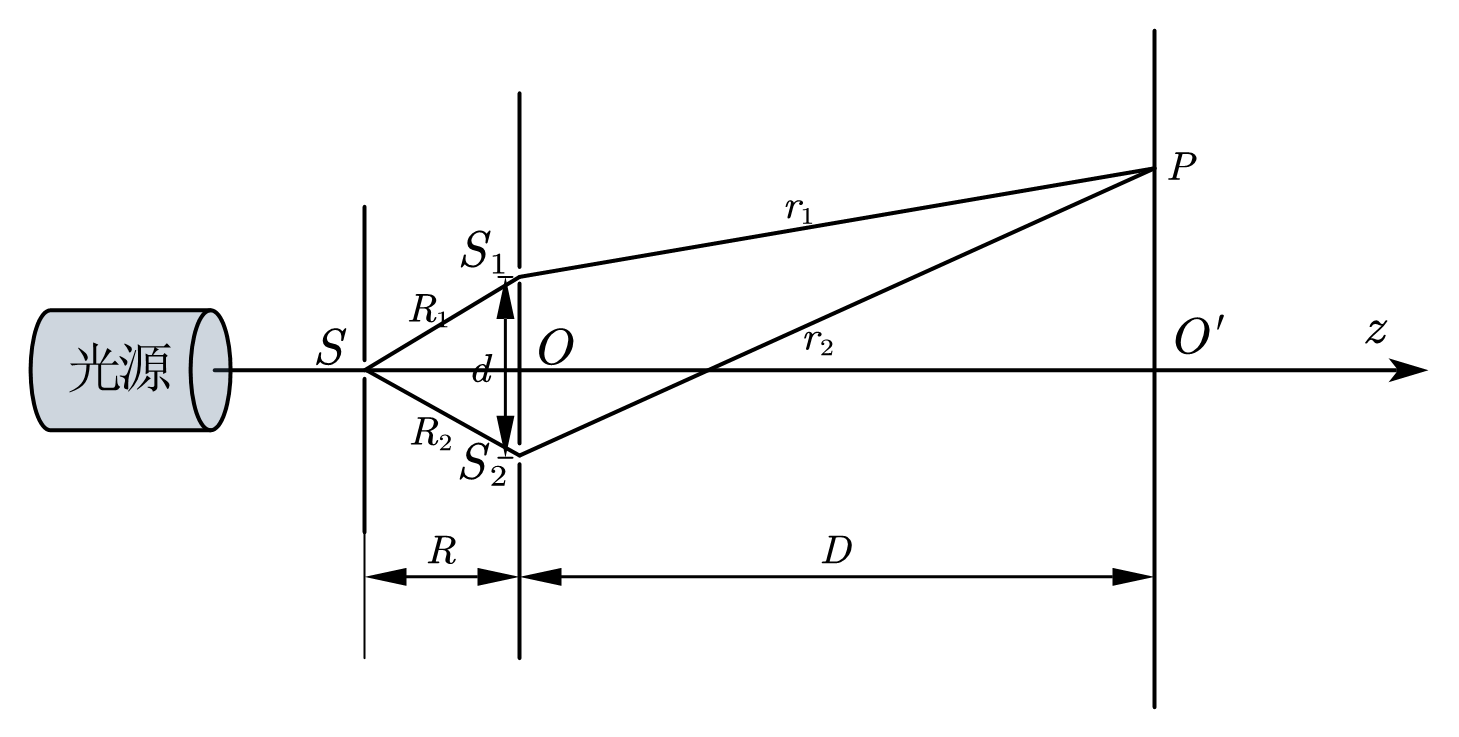
\includegraphics[width=12cm]{./figures/Young_1.png}
\caption{杨氏双缝干涉} \label{Young_fig1}
\end{figure}
在普通单色光源前面放一个开有小孔$S$的屏,作为单色点光源.在$S $的照明范围内再放一个开有两个小孔$S_1,S_2$的屏.按惠更斯原理,$S$将作为两个次波源向前发射次波(球面波),形成交叠的波场.在较远的地方放置一接收屏,屏上可以观测到一组几乎是平行的直线条纹,如\autoref{Young_fig1}(b) .

但这样的亮度太低了.为了提高干涉条纹的亮度,实际中$S,S_1,S_2$用三个互相平行的狭缝($S_1$和$S_2$在同一竖直平面上并都与地面平行,$S$在一竖直平面上且与地面平行,且两竖直平面互相平行)
并且可不用屏幕接收,而代之以目镜直接观测.激光出现以后,人们可以用氦氖激光束直接照明双孔,在屏幕上即可获得一套相当明显的干涉条纹,供许多人同时观看.

\subsection{干涉明暗条纹的位置}
现在来分析,用普通光源做杨氏实验时,由双孔出射的两束光波之间的相位差.设$SS_1=R_1,SS_2=R_2$,用$\varphi_0$代表点波源$S$的初相位,则次波源$S_1,S_2$的初相位分别为
\begin{equation}
\varphi_{10}=\varphi_{0}+\frac{2 \pi}{\lambda} R_{1}, \quad \varphi_{20}=\varphi_{0}+\frac{2 \pi}{\lambda} R_{2}
\end{equation}
从而
\begin{equation}
\varphi_{10}-\varphi_{20}=\frac{2 \pi}{\lambda}\left(R_{1}-R_{2}\right)
\end{equation}
由此可见,两次波之间的相位差与$\varphi_0$无关,即使中$\varphi_0$变了,相位差中$\varphi_{10}-\varphi_{20}$也不变.下面来作一些计算.

令双孔间距为$d$, 屏幕与双孔屏间的距离为$D$,屏幕上横向观测范围为$X$,我们设$d^{2} \ll D^{2}$(这被称为\textbf{远场条件}), $X^{2} \ll D^{2}$(这被称为\textbf{傍轴条件}).

设$S_1$、$S_2$离$S$的距离相等,即$R_1=R_2$, 从而$\varphi_{10}=\varphi_{20}$,为了简化运算,可以取二者皆为$0$,不影响结论.如\autoref{Young_fig1},从线段$S_1S_2$的中点$O$作$z$轴垂直于双孔屏和接收屏.设接收屏上点$P$的横向距离为$X$,$OP$与$z$轴的夹角为$\theta$.在远场条件下,可认为$S_1P\parallel S_2P$, 在傍轴条件下可认为$OP$也与它们平行.从$S_1$作$OP$和$S_2P$的垂线交$S_2P$于$N$.则$\overline{S_2N}$近似等于光程差:
\begin{equation} \label{Young_eq1}
r_{1}-r_{2} \approx \overline{S_{2} N}=d \sin \theta \approx \frac{d x}{D}
\end{equation}
容易得到相位差
\begin{equation}
\delta(P)=\frac{2 \pi\left(r_{1}-r_{2}\right)}{\lambda}=\frac{2 \pi d}{\lambda D} x
\end{equation}
干涉条纹的形状,即等强度线是一组纵向(即与\autoref{Young_fig1}垂直)的平行直线.强度随$\delta(P)$作周期性变化.干涉条纹的间距定义为两条相邻亮纹(强度极大)或两条暗纹(强度极小)之间的距离.因为两条相邻条纹之间的光程差相差$\lambda$, 令\autoref{Young_eq1}中$r_1-r_2=\Delta L=\lambda$,$ x $写成条纹间隔$\Delta x$,则有
\begin{equation}
\Delta x=\frac{\lambda D}{d}
\end{equation}

由上述分析可知,当$P$点处为明纹时,有
\begin{equation}
x=\pm k \frac{D \lambda}{d} \quad k=0,1,2, \cdots
\end{equation}
相应于$k=0$的明纹称为\textbf{零级明纹}或\textbf{中央明纹}.相应于$k=1, k=2, \cdots$的明纹,称为第一级、第二级、……明纹.

当$P$点处为暗纹时,有
\begin{equation}
x=\pm(2 k+1) \frac{D \lambda}{2 d} \quad k=0,1,2, \cdots
\end{equation}

若光源中包含$\lambda_1$和$\lambda_2$两条谱线,则屏上有两套间距不等的条纹同时存在,它们非相干地叠加在一起,如\autoref{Young_fig2}所示.
\begin{figure}[ht]
\centering
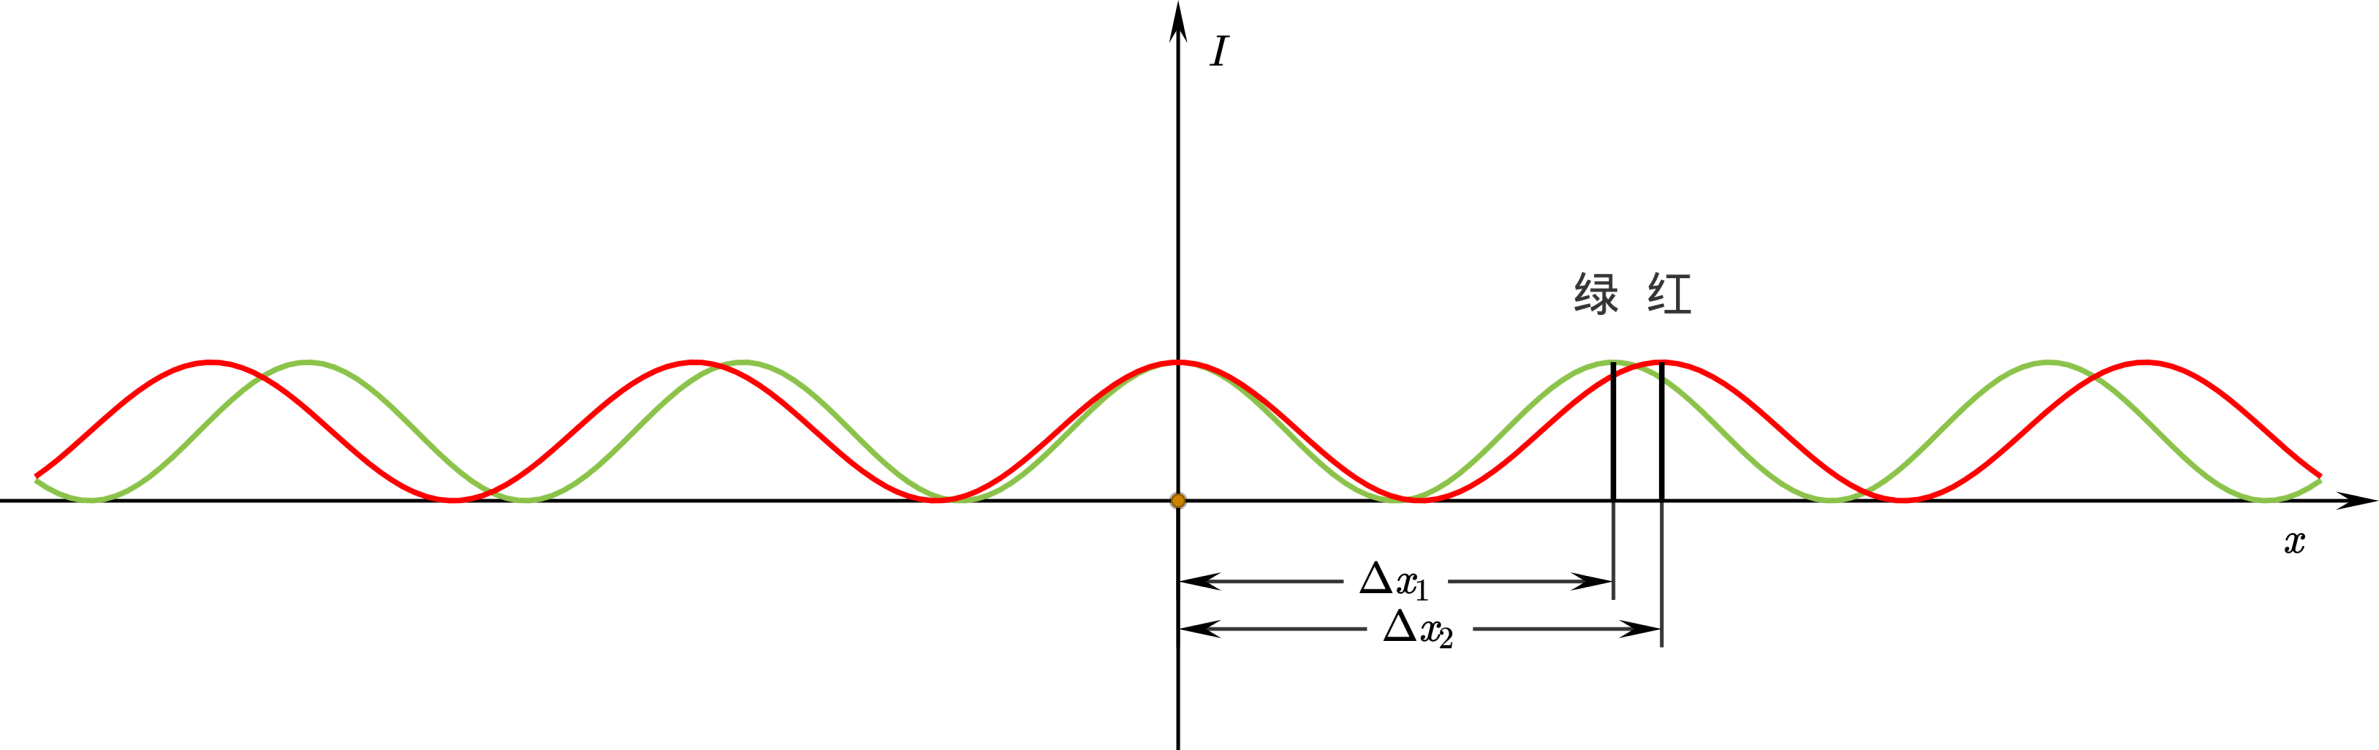
\includegraphics[width=15cm]{./figures/Young_2.png}
\caption{两套不相同颜色干涉条纹不相干叠加} \label{Young_fig2}
\end{figure}
若光源发出的是白光,则在中央零级的白色亮纹两侧,对称地排列着若干条彩色条纹.
\begin{figure}[ht]
\centering
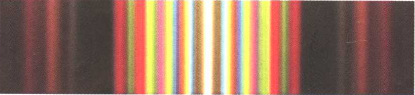
\includegraphics[width=6cm]{./figures/Young_3.png}
\caption{白光的杨氏双缝干涉图样(图片来自维基百科)} \label{Young_fig3}
\end{figure}
